\section{AI use statement}
During the development of this work, we utilized LLMs for grammar correction and occasional text rewriting to improve clarity. LLMs were not used to generate any scientific content, experimental design, data analysis, or intellectual contributions, nor did their assistance influence any of the reported results. 

\section{Analysis of Foundation Models in TCGA-UVM}

\begin{figure}[!ht]
    \centering
    
\includegraphics[width=0.8\linewidth]{figs/um_fm/foundation_model_dendrogram.pdf}
    \caption{Hierarchical clustering based on CKA similarity across 13 foundation models.
    The vertical axis represents the average-linkage distance; lower merge distances indicate greater similarity between learned representation spaces. Blue and orange denote two major model clusters.}
    \label{fig:cka_dendrogram}
\end{figure}

\begin{figure}[!ht]
    \centering
    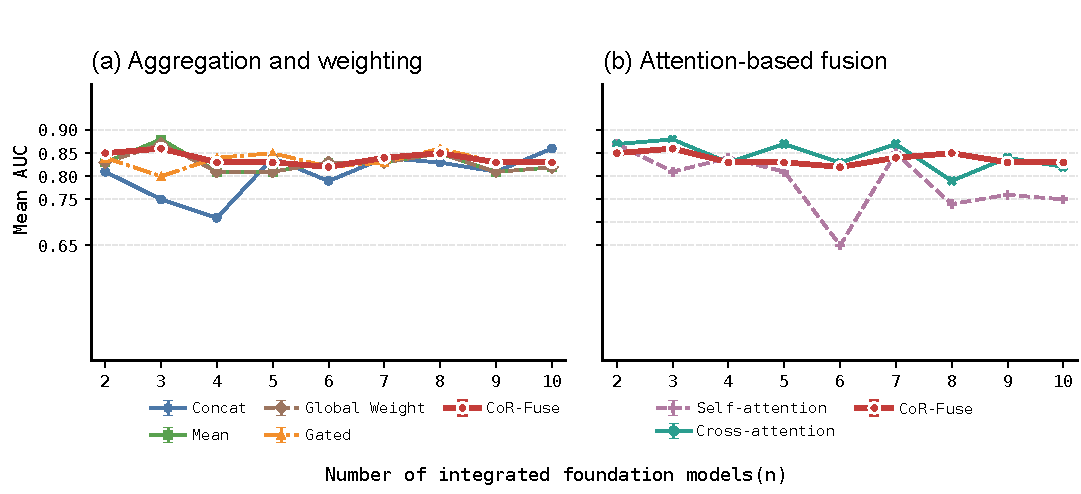
\includegraphics[width=0.8\linewidth]{figs/um_scaling_law/um_scaling_law.pdf}
    \caption{Fusion performance on TCGA-UVM as encoders are added from 2 to 10, ordered by individual validation AUC. Concatenation achieves its highest AUC with 10 integrated foundation models, providing further evidence that fusion performance depends not only on the number of encoders but also on the composition of the representations.}
    \label{fig:scaling_law}
\end{figure}

\begin{table}[!ht]
\centering
\caption{
Comparison of fusion methods on TCGA-UVM.
Results are aggregated across encoder-set sizes $n=2,\ldots,10$, with each composition evaluated using 5-fold cross-validation.}
\label{tab:scaling_law_variance}
\begin{tabular}{lccccc}
\toprule
Method & AUC & AUPRC & F1 & Params(M) & FLOPs(G) \\
\midrule
Mean Fusion & $0.83 \pm 0.02$ & $0.87 \pm 0.02$ & $0.74 \pm 0.01$ & $4.71$ & $52.35$ \\
Concatenation & $0.80 \pm 0.05$ & $0.85 \pm 0.04$ & $0.73 \pm 0.03$ & $6.28$ & $69.85$ \\
Global Weight & $0.83 \pm 0.02$ & $0.86 \pm 0.02$ & $0.74 \pm 0.01$ & $4.71$ & $52.35$ \\
Gated Fusion & $0.83 \pm 0.02$ & $0.87 \pm 0.02$ & $0.75 \pm 0.02$ & $4.71$ & $52.35$ \\
Cross Attention & $0.84 \pm 0.03$ & $0.89 \pm 0.02$ & $0.74 \pm 0.03$ & $6.81$ & $105.16$ \\
Self Attention & $0.79 \pm 0.07$ & $0.83 \pm 0.05$ & $0.72 \pm 0.05$ & $8.38$ & $209.96$ \\
CoR-Fuse & $0.84 \pm 0.01$ & $0.87 \pm 0.01$ & $0.75 \pm 0.02$ & $4.77$ & $52.35$ \\
\bottomrule
\end{tabular}
\end{table}

\begin{figure}[!ht]
    \centering
    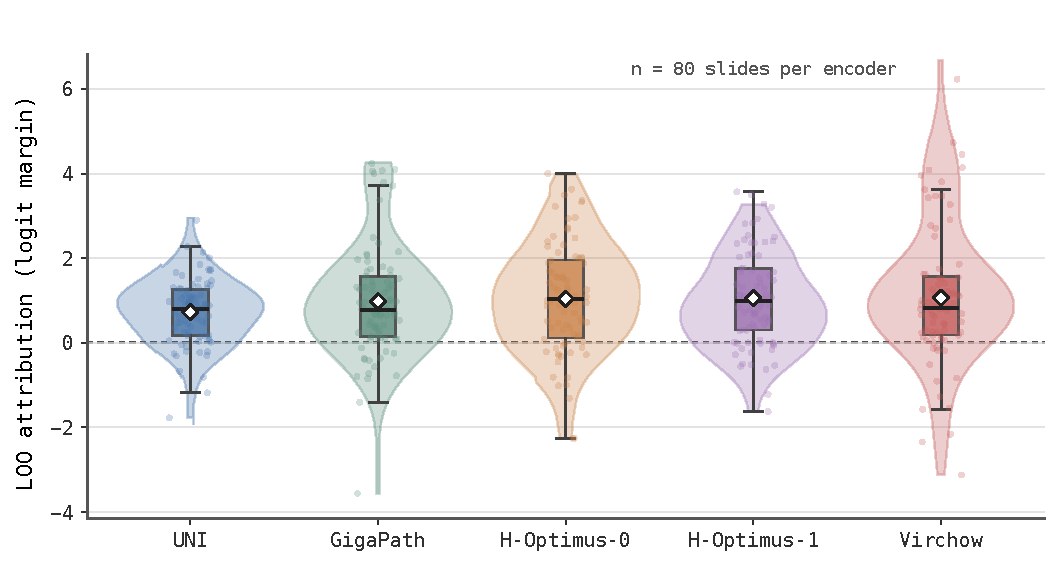
\includegraphics[width=0.8\linewidth]{figs/um_fm/attribution_distribution.pdf}
    \caption{Distribution of leave-one-out (LOO) attribution scores \(C_m^{\text{LOO}}\) across 80 TCGA-UVM slides for the encoder set \{UNI, GigaPath, H-optimus-0, H-optimus-1, Virchow\}.
    This encoder set is selected from the evaluated foundation models for visualization and does not correspond to a specific composition used in the main experiments.
    Each boxplot shows the distribution of attribution values across slides for encoder $m$. Positive and negative attributions indicate favorable and adverse contributions to the downstream prediction.}
    \label{fig:attribution_distribution}
\end{figure}

\begin{figure}[!ht]
    \centering
    
\includegraphics[width=0.8\linewidth]{figs/um_fm/mean_abs_spearman_heatmap.pdf}
    \caption{Mean absolute feature-level Spearman correlation $R_{ij}$ across the 13 pathology encoders on TCGA-UVM. The weak and compressed range of Spearman correlations, despite the broader CKA range, highlights that global geometric similarity and feature-level statistical correspondence capture different aspects of encoder relationships.}
    \label{fig:all_Spearman_heatmap}
\end{figure}

\begin{table}[!ht]
    \centering
    \caption{Single foundation model performance on TCGA-UVM D3/M3 classification.
    The results, ordered by AUC and the results are reported as mean $\pm$ standard deviation over five folds.}
    \label{tab:uvm_all_fm_performance}
    \begin{tabular}{lccc}
    \toprule
    Model & AUC & AUPRC & F1 \\
    \midrule
    H-optimus-1 &$\mathbf{0.84 \pm 0.15}$ &$0.86 \pm 0.14$ &$0.75 \pm 0.18$ \\
    Virchow2 &$0.83 \pm 0.12$ &$0.85 \pm 0.14$ &$\mathbf{0.78 \pm 0.11}$ \\
    H-optimus-0 &$0.83 \pm 0.14$ &$\mathbf{0.86 \pm 0.13}$ &$0.76 \pm 0.14$ \\
    GigaPath &$0.79 \pm 0.16$ &$0.83 \pm 0.14$ &$0.70 \pm 0.17$ \\
    CONCH &$0.78 \pm 0.14$ &$0.82 \pm 0.15$ &$0.73 \pm 0.17$ \\
    CONCH-v1.5 &$0.76 \pm 0.16$ &$0.78 \pm 0.17$ &$0.72 \pm 0.19$ \\
    Phikon &$0.76 \pm 0.21$ &$0.81 \pm 0.18$ &$0.70 \pm 0.16$ \\
    UNI-v2 &$0.76 \pm 0.24$ &$0.81 \pm 0.19$ &$0.69 \pm 0.18$ \\
    Virchow &$0.74 \pm 0.17$ &$0.75 \pm 0.18$ &$0.70 \pm 0.14$ \\
    Phikon-v2 &$0.74 \pm 0.19$ &$0.78 \pm 0.20$ &$0.62 \pm 0.20$ \\
    Hibou-L &$0.73 \pm 0.17$ &$0.82 \pm 0.13$ &$0.67 \pm 0.12$ \\
    UNI &$0.72 \pm 0.19$ &$0.75 \pm 0.21$ &$0.67 \pm 0.27$ \\
    Midnight-12k &$0.59 \pm 0.25$ &$0.67 \pm 0.20$ &$0.62 \pm 0.15$ \\
    \bottomrule
    \end{tabular}
\end{table}

\clearpage
\section{Experiments on TCGA-UVM}

\begin{table}[!ht]
\centering
\caption{Representation similarity and individual-FM predictive performance for three representative five-encoder compositions on TCGA-UVM.
Notably, representation similarity does not directly track individual predictive strength.
For example, the high-similarity and heterogeneous compositions exhibit substantially different mean pairwise CKA values (0.930 vs 0.777), yet their best individual-FM AUCs remain similar (0.840 vs 0.830).}
\label{tab:composition_summary}
\begin{tabular}{lccc}
\toprule
Encoder composition & Mean pairwise CKA & Mean individual AUC & Best individual AUC \\
\midrule
High-similarity & $0.930 $ & $0.784$ & $0.840$ \\
Intermediate-similarity & $0.854 $ & $0.804$ & $0.840$ \\
Heterogeneous  & $0.777$ & $0.782 $ & $0.830$ \\
\bottomrule
\end{tabular}
\end{table}

\begin{table}[htbp]
\centering
\caption{Fusion performance of existing methods under \{H-optimus-1, H-optimus-0, Virchow2, UNI-v2, CONCH-v1.5\} composition on TCGA-UVM.}
\label{tab:uvm_existing_methods}
\begin{tabular}{lccccc}
\toprule
Method & AUC & AUPRC & F1 & Params(M) & FLOPs(G)\\
\midrule
Mean Fusion & $0.83 \pm 0.04$ & $0.87 \pm 0.04$ & $0.73 \pm 0.06$ & $4.27$ & $47.47$\\
Cross Attention & $0.79 \pm 0.04$ & $0.84 \pm 0.03$ & $0.70 \pm 0.05$ & $6.37$ & $94.40$\\
Meta-Encoder & $0.60 \pm 0.17$ & $0.66 \pm 0.10$ & $0.60 \pm 0.19$ & $25.76$ & $533.97$\\
FuseCPath & $0.70 \pm 0.03$ & $0.76 \pm 0.02$ & $0.63 \pm 0.11$ &$7.42$ &$3.34$\\
CoR-Fuse & $\mathbf{0.84 \pm 0.01}$ & $\mathbf{0.87 \pm 0.03}$ & $\mathbf{0.77 \pm 0.03}$ & $4.34$ & $47.47$\\
\bottomrule
\end{tabular}
\end{table}

\begin{table}[htbp]
\centering
\caption{Fusion performance on TCGA-UVM under the fixed encoder composition of \{H-optimus-0, Virchow2, UNI, GigaPath, CONCH-v1.5\}.}
\label{tab:elf_uvm}
\begin{tabular}{lccc}
\toprule
Method & AUC & AUPRC & F1\\
\midrule
Mean Fusion & $0.81 \pm 0.01$ & $\mathbf{0.84 \pm 0.02}$ & $0.72 \pm 0.02$\\
Concatenation & $0.74 \pm 0.02$ & $0.77 \pm 0.03$ & $0.63 \pm 0.11$\\
Global Weight & $0.81 \pm 0.00$ & $\mathbf{0.84 \pm 0.02}$ & $0.72 \pm 0.02$ \\
Gated Fusion & $0.81 \pm 0.03$ & $0.82 \pm 0.05$ & $\mathbf{0.74 \pm 0.04}$\\
Cross Attention & $0.79 \pm 0.02$ & $0.83 \pm 0.02$ & $0.68 \pm 0.05$ \\
ELF & $0.80 \pm 0.02$ & $0.83 \pm 0.03$ & $\mathbf{0.74 \pm 0.02}$ \\
CoR-Fuse & $\mathbf{0.82 \pm 0.04}$ & $0.83 \pm 0.02$ & $0.73 \pm 0.03$ \\
\bottomrule
\end{tabular}
\end{table}

\clearpage
\subsection{Experimental Results of Five Heterogeneous Encoders}
\label{sec:high cka}

\begin{figure}[!ht]
    \centering
    
\includegraphics[width=0.8\linewidth]{figs/um_n5_cka_range_max/cka_abs_interaction_quadrants.pdf}
    \caption{Pairwise CKA versus mean absolute task-level interaction $|I_{ij}|$ for the heterogeneous five-encoder composition on TCGA-UVM. The scatter plot includes encoder pairs with relatively high CKA similarity ($>0.77$) and varying interaction magnitudes ($>0.18$), suggesting that geometric similarity alone may not fully characterize task-level relationships between encoder representations.}
    \label{fig:n5_diversity_max_quadrants}
\end{figure}

\begin{table}[!ht]
\centering
\caption{Fusion performance under the heterogeneous five-encoder composition \{Hibou-L, Virchow2, CONCH-v1.5, UNI-v2, H-optimus-0\} on TCGA-UVM. In contrast to the high-similarity composition (Table~\ref{tab:uvm_high_similarity}), where attention-based methods perform better, the observed differences suggest that fusion effectiveness may vary across representation compositions.}
\label{tab:uvm_high_diversity}
\begin{tabular}{lccc}
\toprule
Method & AUC & AUPRC & F1 \\
\midrule
Mean Fusion & $0.84 \pm 0.11$ & $0.88 \pm 0.09$ & $0.75 \pm 0.15$ \\
Concatenation & $0.84 \pm 0.09$ & $0.87 \pm 0.09$ & $0.73 \pm 0.09$ \\
Global Weight & $\mathbf{0.85 \pm 0.11}$ & $\mathbf{0.89 \pm 0.09}$ & $\mathbf{0.78 \pm 0.11}$ \\
Cross Attention & $0.81 \pm 0.13$ & $0.84 \pm 0.12$ & $0.70 \pm 0.24$ \\
Self Attention & $0.78 \pm 0.13$ & $0.83 \pm 0.10$ & $0.72 \pm 0.13$ \\
Gated Fusion & $0.81 \pm 0.13$ & $0.85 \pm 0.11$ & $0.74 \pm 0.16$ \\
CoR-Fuse & $0.83 \pm 0.11$ & $0.88 \pm 0.10$ & $0.73 \pm 0.15$ \\
\bottomrule
\end{tabular}
\end{table}

\clearpage
\subsection{Experimental Results of Five High-Similarity Encoders}
\label{sec:high similarity}

\begin{figure}[!ht]
    \centering
    
\includegraphics[width=0.8\linewidth]{figs/um_n5_high_redundancy_group/cka_abs_interaction_quadrants.pdf}
    \caption{Pairwise CKA versus mean absolute task-level interaction $|I_{ij}|$ for the high-similarity five-encoder composition. The highly similar H-optimus-0 and H-optimus-1 pair exhibits a large interaction magnitude, illustrating that high geometric similarity can coexist with strong task-level interaction. The direction of this interaction is examined separately using signed interaction statistics.}
    \label{fig:n5_high_redundancy_quadrants}
\end{figure}

\begin{table}[!ht]
\centering
\caption{Fusion performance under the high-similarity five-encoder composition \{H-optimus-0, H-optimus-1, UNI, GigaPath, Phikon-v2\}. The ranking of fusion strategies reverses relative to Table~\ref{tab:uvm_high_diversity}: attention-based methods perform best in this setting, whereas simpler aggregation methods lag behind. This pattern supports our central observation that no single fusion strategy consistently dominates across encoder compositions.}
\label{tab:uvm_high_similarity}
\begin{tabular}{lccc}
\toprule
Method & AUC & AUPRC & F1 \\
\midrule
Mean Fusion & $0.79 \pm 0.18$ & $0.82 \pm 0.17$ & $0.72 \pm 0.18$ \\
Concatenation & $0.83 \pm 0.09$ & $0.88 \pm 0.10$ & $0.76 \pm 0.13$ \\
Global Weight & $0.79 \pm 0.18$ & $0.82 \pm 0.17$ & $0.72 \pm 0.18$ \\
Cross Attention & $\mathbf{0.86 \pm 0.12}$ & $0.88 \pm 0.11$ & $\mathbf{0.81 \pm 0.09}$ \\
Self Attention & $0.85 \pm 0.11$ & $\mathbf{0.88 \pm 0.08}$ & $0.76 \pm 0.10$ \\
Gated Fusion & $0.83 \pm 0.15$ & $0.86 \pm 0.12$ & $0.74 \pm 0.16$ \\
CoR-Fuse & $0.83 \pm 0.11$ & $0.87 \pm 0.11$ & $0.74 \pm 0.17$ \\
\bottomrule
\end{tabular}
\end{table}

\clearpage
\subsection{Analysis Results of Five Intermediate-Similarity Encoders}
\label{sec:balanced}

\begin{figure}[!ht]
    \centering
    
\includegraphics[width=0.8\linewidth]{figs/um_n5_per_high_cka_high/cka_abs_interaction_quadrants.pdf}
    \caption{Pairwise CKA versus mean absolute task-level interaction $|I_{ij}|$ for the intermediate-similarity five-encoder composition. The distribution across different CKA-interaction regimes suggests that geometric similarity alone may not fully characterize task-level relationships between pathology foundation encoders.}
    \label{fig:n5_balanced_quadrants}
\end{figure}

\begin{table}[htbp]
\centering
\caption{Fusion performance under an intermediate-similarity five-encoder composition on TCGA-UVM.}
\label{tab:uvm_n5_balanced_group}
\begin{tabular}{lccccc}
\toprule
Method & AUC & AUPRC & F1\\
\midrule
Mean Fusion & $0.83 \pm 0.04$ & $0.87 \pm 0.04$ & $0.73 \pm 0.06$\\
Concatenation & $0.77 \pm 0.05$ & $0.83 \pm 0.03$ & $0.69 \pm 0.04$\\
Global Weight & $0.83 \pm 0.04$ & $0.87 \pm 0.05$ & $0.73 \pm 0.06$\\
Gated Fusion & $0.83 \pm 0.03$ & $0.86 \pm 0.03$ & $0.72 \pm 0.05$\\
Cross Attention & $0.79 \pm 0.04$ & $0.84 \pm 0.03$ & $0.70 \pm 0.05$\\
Self Attention & $0.80 \pm 0.08$ & $0.85 \pm 0.09$ & $0.70 \pm 0.04$\\
CoR-Fuse & $\mathbf{0.84 \pm 0.01}$ & $\mathbf{0.87 \pm 0.03}$ & $\mathbf{0.77 \pm 0.03}$\\
\bottomrule
\end{tabular}
\end{table}

\clearpage
\section{Experiments on TCGA-BLCA}
\label{sec:blca_results}

\begin{table}[!ht]
    \centering
    \caption{Single foundation model performance on TCGA-BLCA TP53 mutation status classification. Results averaged over 5-fold cross-validation.}
    \label{tab:blca_all_fm_performance}
    \begin{tabular}{lccc}
    \toprule
    Model & AUC & AUPRC & F1 \\
    \midrule
    Phikon &$\mathbf{0.73 \pm 0.01}$ &$\mathbf{0.72 \pm 0.09}$ &$\mathbf{0.66 \pm 0.08}$ \\
    Virchow2 &$0.71 \pm 0.06$ &$0.70 \pm 0.07$ &$0.60 \pm 0.09$ \\
    GigaPath &$0.68 \pm 0.04$ &$0.65 \pm 0.12$ &$0.64 \pm 0.11$ \\
    UNI &$0.67 \pm 0.04$ &$0.68 \pm 0.14$ &$0.61 \pm 0.11$ \\
    Midnight-12k &$0.62 \pm 0.06$ &$0.63 \pm 0.13$ &$0.61 \pm 0.13$ \\
    \bottomrule
    \end{tabular}
\end{table}

\begin{table}[!ht]
\centering
\caption{Representation similarity and individual-model performance for \{UNI, Virchow2, Midnight-12k, GigaPath, Phikon\} composition on TCGA-BLCA.}
\label{tab:composition_blca}
\begin{tabular}{lcc}
\toprule
Mean pairwise CKA & Mean individual AUC & Best individual AUC \\
\midrule
$0.750 $ & $0.682$ & $0.730$ \\
\bottomrule
\end{tabular}
\end{table}

\begin{figure}[!ht]
    \centering
    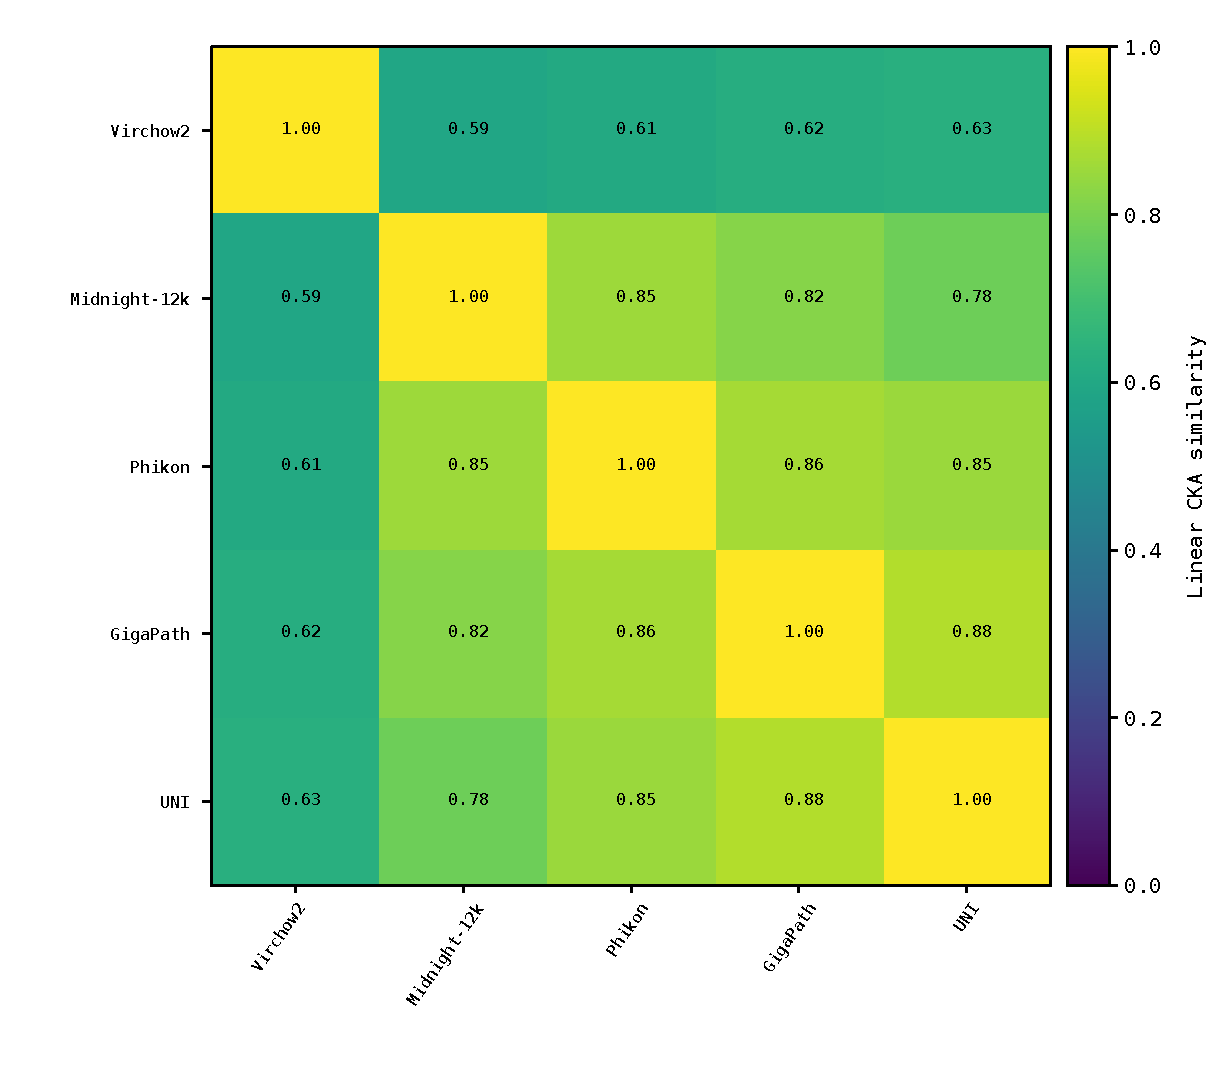
\includegraphics[width=0.8\linewidth]{figs/blca/pairwise_linear_cka_similarity_matrix.pdf}
    \caption{Pairwise CKA similarity matrix for five-encoder composition on TCGA-BLCA. Each entry reports the CKA similarity between a pair of foundation-model representations.}
    \label{fig:blca_cka_matrix}
\end{figure}

\begin{figure}[!ht]
    \centering
    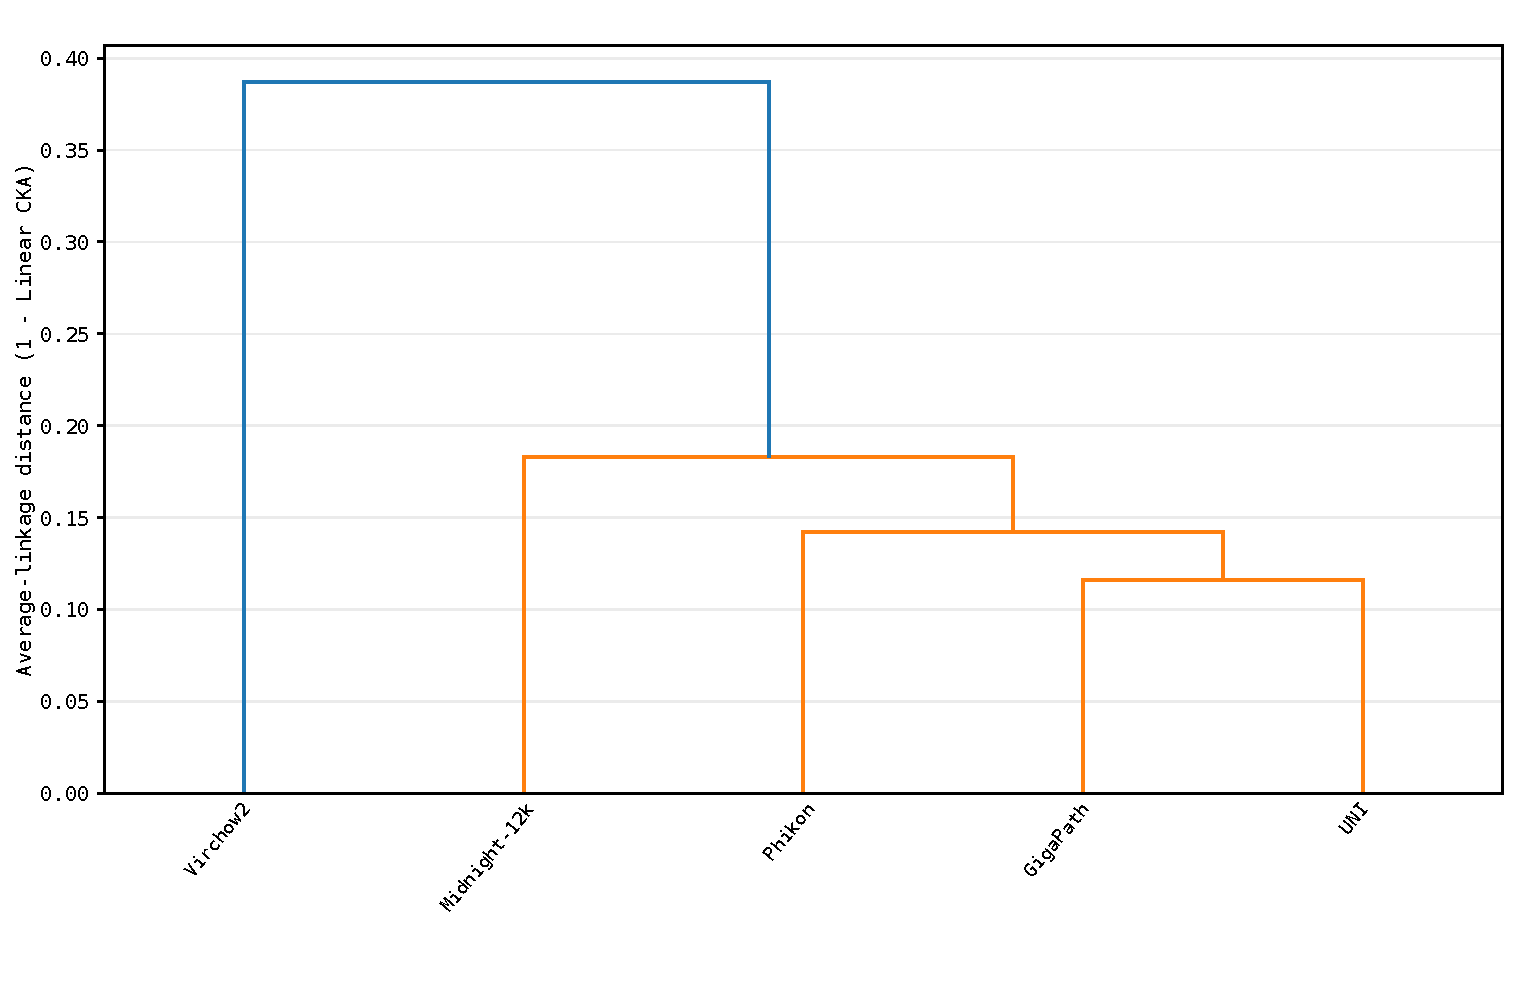
\includegraphics[width=0.8\linewidth]{figs/blca/foundation_model_dendrogram.pdf}
    \caption{Hierarchical clustering of the five foundation-model representations on TCGA-BLCA based on pairwise CKA similarity. Virchow2 forms a relatively distinct branch, indicating lower representational similarity with the other evaluated encoders.}
    \label{fig:blca_dendrogram}
\end{figure}

\begin{figure}[!ht]
    \centering
    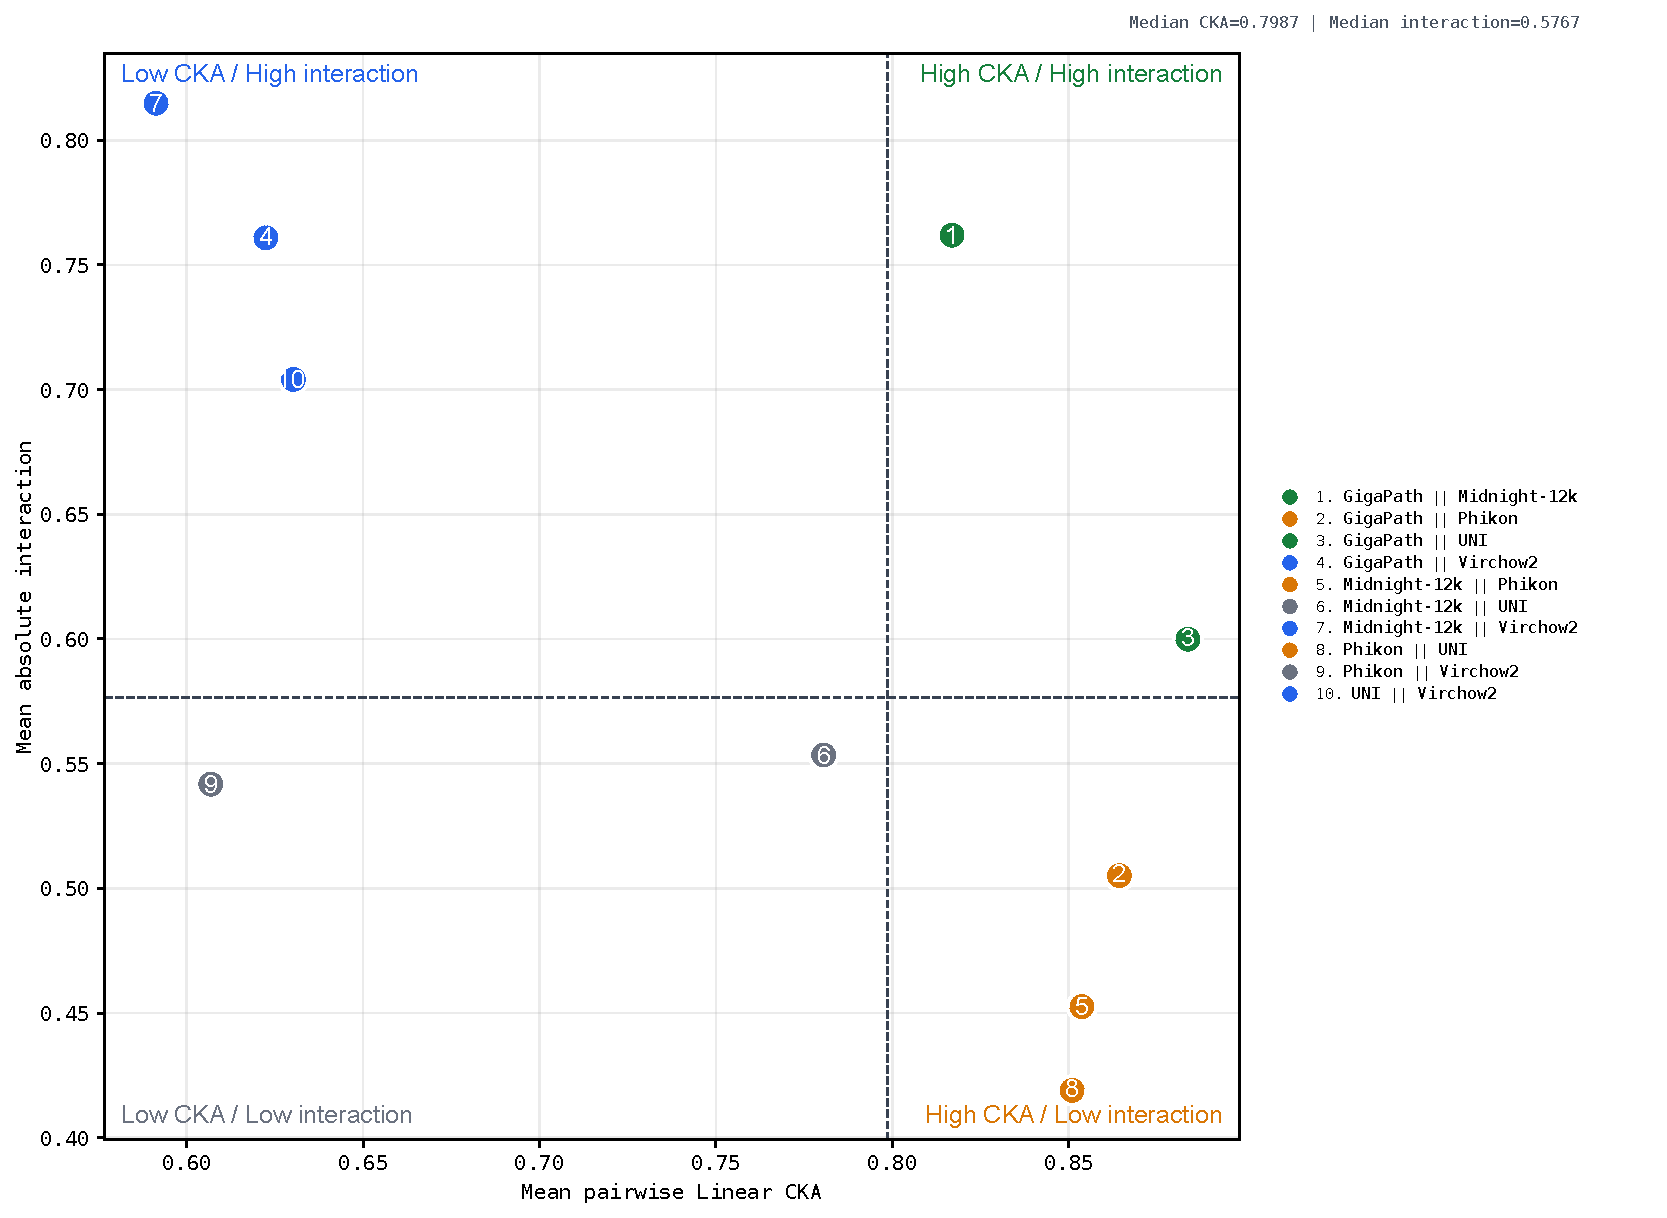
\includegraphics[width=0.8\linewidth]{figs/blca/cka_abs_interaction_quadrants.pdf}
    \caption{Pairwise CKA versus mean absolute task-level interaction $|I_{ij}|$ for the five-encoder composition on TCGA-BLCA. Each point represents a pair of foundation models, with CKA measuring representational similarity and $|I_{ij}|$ measuring the magnitude of their task-level interaction.}
    \label{fig:blca_quadrants}
\end{figure}

\begin{figure}[!ht]
    \centering
    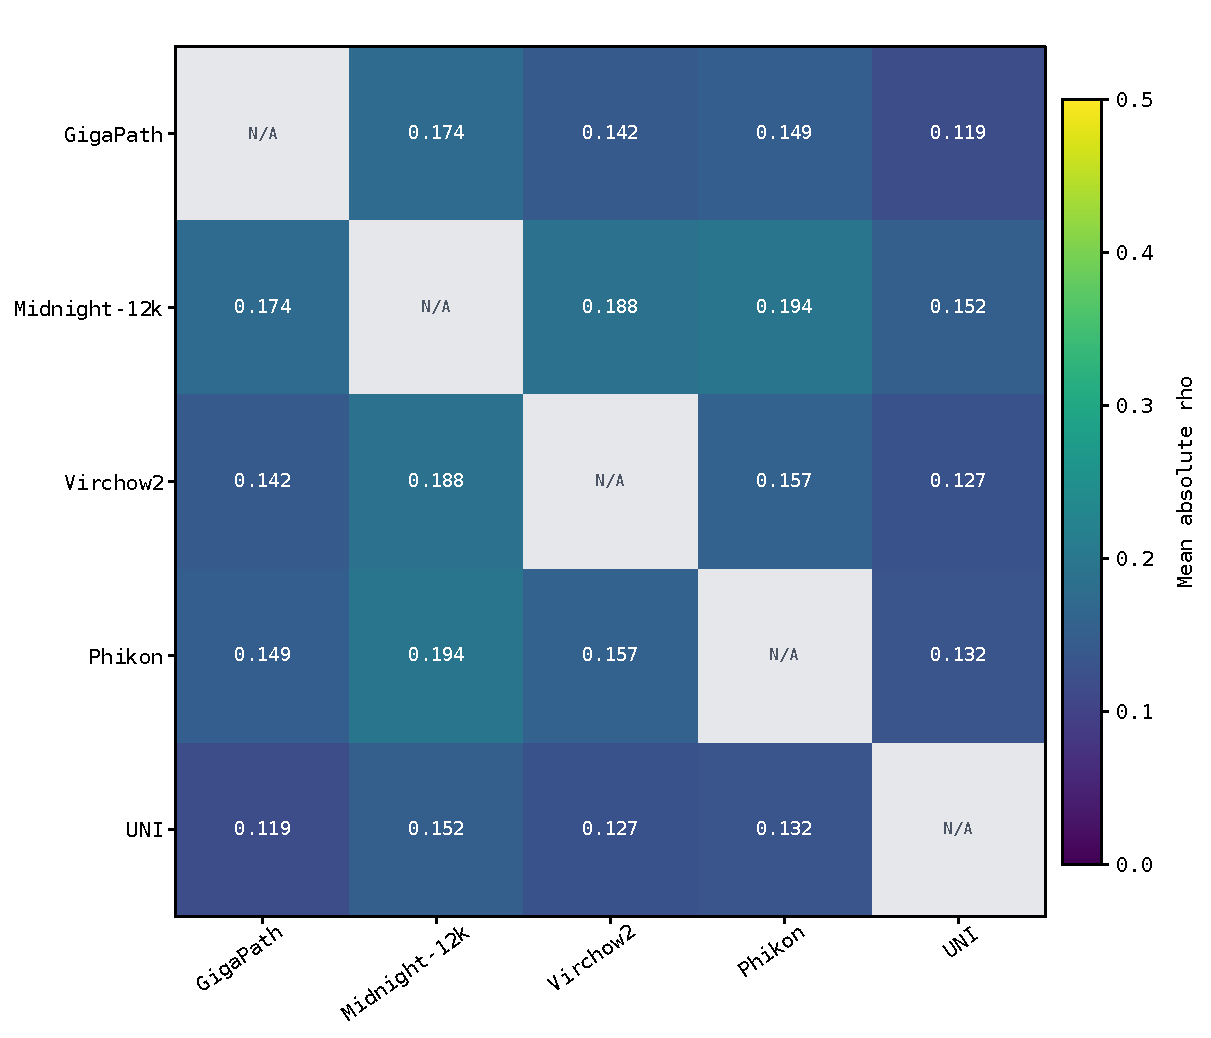
\includegraphics[width=0.8\linewidth]{figs/blca/mean_abs_spearman_heatmap.pdf}
    \caption{Mean absolute feature-level Spearman correlation for five-encoder composition on TCGA-BLCA. Each entry summarizes the mean absolute Spearman correlation between a pair of encoder representations at the feature level.}
    \label{fig:blca_heatmap}
\end{figure}


\clearpage
\section{Implementation Details}
\label{implemented details}
All experiments were implemented in PyTorch and run on one NVIDIA GeForce RTX 4090 GPU.
We conducted experiments using three random seeds (42, 35, and 2026) with 5-fold cross-validation to assess reproducibility. The warm start stage was optimized for 20 epochs with a learning rate of \(1\times10^{-4}\). The subsequent fusion stage was trained for 80 epochs with the same learning rate. For scoring, we used a lightweight two-layer MLP (1024 $\rightarrow$ 64 $\rightarrow$ 1).

To align heterogeneous foundation-model embeddings, we employ an encoder-specific lightweight projection head for each encoder. Each head consists of a linear projection to a shared 512-dimensional space, followed by LayerNorm and dropout (\(p=0.1\)); no additional nonlinear activation is used. The projection heads are independently parameterized across encoders. Linear layers are Xavier-normal initialized with zero biases, while LayerNorm scales and biases are initialized to one and zero, respectively.
The reported FLOPs account only for downstream projection, routing, and aggregation operations applied to pre-extracted embeddings, excluding the forward passes of the frozen foundation-model backbones.

For a fair comparison across ablation variants, we keep the total optimization budget consistent across all variants. The full CoR-Fuse model is trained for 20 epochs in Stage 1 and 80 epochs in Stage 2, for a total of 100 epochs. For the w/o Warm Start variant, the model is trained for the same total of 100 epochs from random initialization, with the corresponding routing-stage optimization performed throughout training.
Thus, differences between the warm-start and w/o Warm Start variants are attributable to the initialization strategy rather than a difference in the total number of training epochs.

\section{Experimental Results of Multiple Downstream Heads}
\begin{table}[!ht]
\centering
\caption{Performance of different fusion strategies and downstream heads on TCGA-UVM using the representative three-encoder composition \{H-optimus-0, Virchow2, CONCH\}.
CoR-Fuse achieves the highest AUC and AUPRC with ABMIL among the evaluated CoR-Fuse variants, while simple fusion strategies remain competitive with this three-encoder composition.}
\label{tab:downstream_heads}
\begin{tabular}{lccc}
\toprule
Method & AUC & AUPRC & F1 \\
\midrule
Mean Fusion & $0.83 \pm 0.11$ & $0.86 \pm 0.09$ & $0.68 \pm 0.16$ \\
Concatenation & $0.81 \pm 0.10$ & $0.87 \pm 0.05$ & $\mathbf{0.75 \pm 0.08}$ \\
Global Weight & $0.83 \pm 0.11$ & $0.86 \pm 0.10$ & $0.69 \pm 0.18$ \\
Cross Attention & $0.78 \pm 0.09$ & $0.83 \pm 0.09$ & $0.72 \pm 0.11$ \\
Gated Fusion & $0.70 \pm 0.27$ & $0.74 \pm 0.24$ & $0.73 \pm 0.12$ \\
CoR-Fuse(ABMIL) & $\mathbf{0.85 \pm 0.08}$ & $\mathbf{0.89 \pm 0.09}$ & $0.74 \pm 0.19$ \\
CoR-Fuse(TransMIL) & $0.80 \pm 0.16$ & $0.84 \pm 0.13$ & $0.72 \pm 0.17$ \\
CoR-Fuse(MLP) & $0.71 \pm 0.20$ & $0.76 \pm 0.17$ & $0.61 \pm 0.23$ \\
CoR-Fuse(GNN) & $0.75 \pm 0.18$ & $0.76 \pm 0.18$ & $0.70 \pm 0.16$ \\
\bottomrule
\end{tabular}
\end{table}

\section{Detailed Information of Compared Fusion Methods}
\label{sec:contrast_method}

\subsection{Mean Fusion}
Uniform mean fusion assigns an equal weight of $1/M$ to every encoder:
\begin{equation}
\mathbf{Z}_p =
\frac{1}{M}\sum_{m=1}^{M}\mathbf{H}_{m,p}.
\end{equation}
This parameter-free baseline assumes that all encoders contribute equally.

\subsection{Concatenation}
Feature concatenation is performed on the projected latent representations $\mathbf{H}_{M,p}$ into a joint 512 $M-$ dimensional vector prior to downstream bag aggregation:
\begin{equation}
\mathbf{Z}_p =
[\mathbf{H}_{1,p};\mathbf{H}_{2,p};\ldots;\mathbf{H}_{M,p}]
\in\mathbb{R}^{512M}.
\end{equation}

\subsection{Global Weight Fusion}
This method learns a single set of encoder weights shared across all slides and patches:
\begin{equation}
\mathbf{Z}_p =
\sum_{m=1}^{M}w_m\mathbf{H}_{m,p},
\qquad
\mathbf{w}=\operatorname{softmax}(\mathbf{b}),
\quad
\mathbf{b}\in\mathbb{R}^{M}.
\end{equation}
The encoder-weight logits are optimized jointly with the downstream network.
This baseline tests whether a fixed global preference over encoders can improve upon uniform averaging.

\subsection{Gated Fusion}
Gated fusion produces slide-specific encoder weights from slide-level encoder descriptors.
For encoder $m$, its slide-level descriptor is obtained by mean pooling its patch embeddings:
\begin{equation}
\mathbf{\mu}_m^{(n)}
=
\frac{1}{P_n}
\sum_{p=1}^{P_n}\mathbf{H}_{m,p}^{(n)}.
\end{equation}
A shared linear gate produces an encoder score:
\begin{equation}
g_m
=
\sigma\left(
\mathbf{a}^{\top}\mathbf{\mu}_m+b
\right),
\end{equation}
where $\mathbf{a}\in\mathbb{R}^{512}$ and $b\in\mathbb{R}$ are shared across encoders.
The scores are normalized across encoders:
\begin{equation}
w_m
=
\frac{g_m}
{\sum_{j=1}^{M}g_j}.
\end{equation}
The resulting weights are applied to all patches of the corresponding slide.
Unlike global weighting, this formulation allows encoder weights to vary across slides while remaining shared across patches within each slide.
The gate computes each encoder score from its own slide-level descriptor without explicitly modeling pairwise relationships among encoders.

\section{Ablation Study}
\label{sec:ablation_study}

\begin{table}[!ht]
\centering
\caption{
Comparison of routing weights with and without the consensus component.
The Gini coefficient measures the concentration of routing weights across encoders, while the per-encoder weights characterize encoder utilization.
}
\label{tab:weight_compare_woconsensus}
\begin{tabular}{lcc}
\toprule
\multicolumn{3}{c}{\textbf{Overall Routing Concentration}} \\
\midrule
Setting & Mean Gini & Normalized Gini \\
\midrule
With Consensus    & $0.2269 \pm 0.0752$ & $0.2836$ \\
Without Consensus & $0.2291 \pm 0.1095$ & $0.2863$ \\
\midrule
\multicolumn{3}{c}{\textbf{Per-Encoder Routing Weight}} \\
\midrule
Foundation Model & With Consensus & Without Consensus \\
\midrule
Phikon       & $0.3194 \pm 0.0973$ & $0.3048 \pm 0.1303$ \\
GigaPath     & $0.2048 \pm 0.0521$ & $0.2101 \pm 0.0723$ \\
UNI          & $0.1929 \pm 0.0484$ & $0.1768 \pm 0.0630$ \\
Virchow2     & $0.1459 \pm 0.0783$ & $0.1588 \pm 0.0757$ \\
Midnight-12k & $0.1371 \pm 0.0441$ & $0.1494 \pm 0.0630$ \\
\bottomrule
\end{tabular}
\end{table}

\section{Understanding the Effect of Mean-Fusion Warm-Start}
\label{sec:warm_start}

We further investigate why initializing CoR-Fuse from a mean-fusion model facilitates optimization.
During Stage 1, encoder-specific projection heads and the downstream prediction head are optimized using a uniform aggregation strategy.

Let $\theta^{(1)}$ and $\phi^{(1)}$ denote the encoder-specific projection parameters and downstream prediction-head parameters, respectively, after Stage 1. Let $\theta^{(2)}$ and $\phi^{(2)}$ denote the corresponding parameters at the beginning of Stage 2. We initialize Stage 2 by transferring the parameters learned in Stage 1:
\begin{equation}
\theta^{(2)} \leftarrow \theta^{(1)},
\qquad
\phi^{(2)} \leftarrow \phi^{(1)}.
\end{equation}
The uniform aggregation is then replaced by slide-specific routing.

This initialization provides two optimization advantages.
First, the projection heads already map heterogeneous encoder features into a task-aligned latent space.
Second, the downstream prediction head starts from parameters adapted to a predictive fused representation.
Therefore, the routing stage mainly focuses on refining encoder contributions rather than jointly learning representation projection, prediction, and routing from random initialization.

Moreover, mean-fusion initialization provides a permutation-symmetric starting point, where all encoders receive equal initial importance before task-specific evidence is introduced.
This reduces the risk of unstable early routing behavior caused by randomly initialized projections and routing scores, which is particularly relevant in the low-sample regime.

\begin{figure}[!ht]
    \centering
    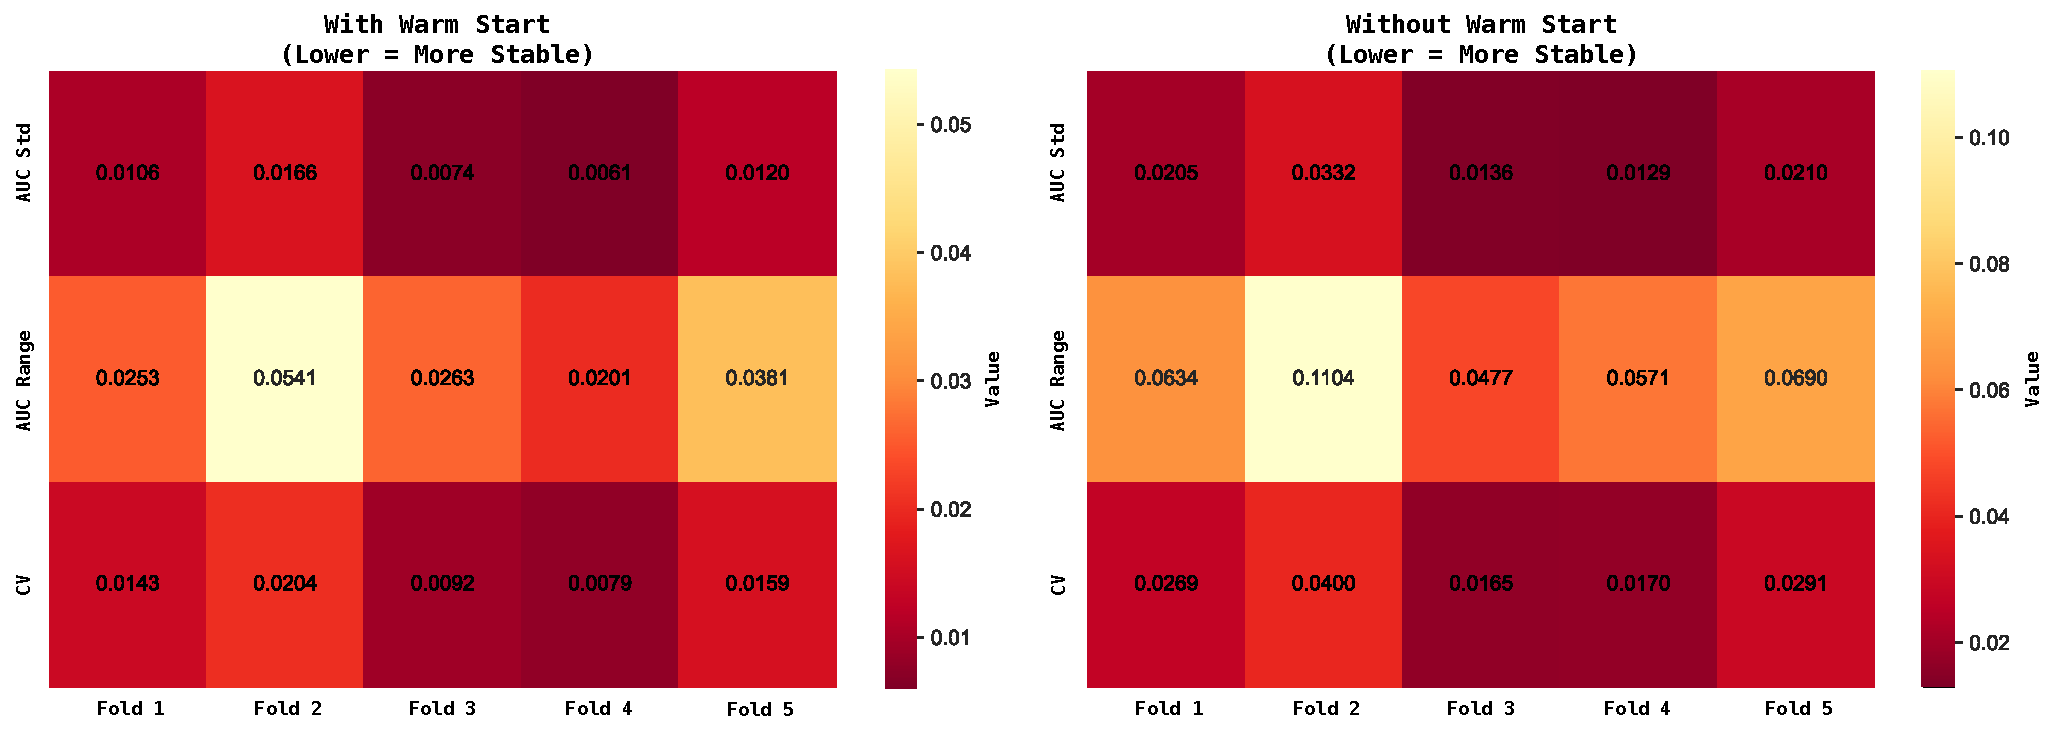
\includegraphics[width=1.0\linewidth]{figs/blca/warm_start/stability_heatmap.pdf}
    \caption{Heatmaps of three stability metrics (AUC Std, AUC Range, and CV) across five CV folds for models with and without warm start. Smaller values correspond to greater stability. Every metric value in the without-warm-start condition is higher than that in the warm-start setting, verifying the stabilizing effect of warm start.}
    \label{fig:warmstart_stability_heatmap}
\end{figure}

\begin{figure}[!ht]
    \centering
    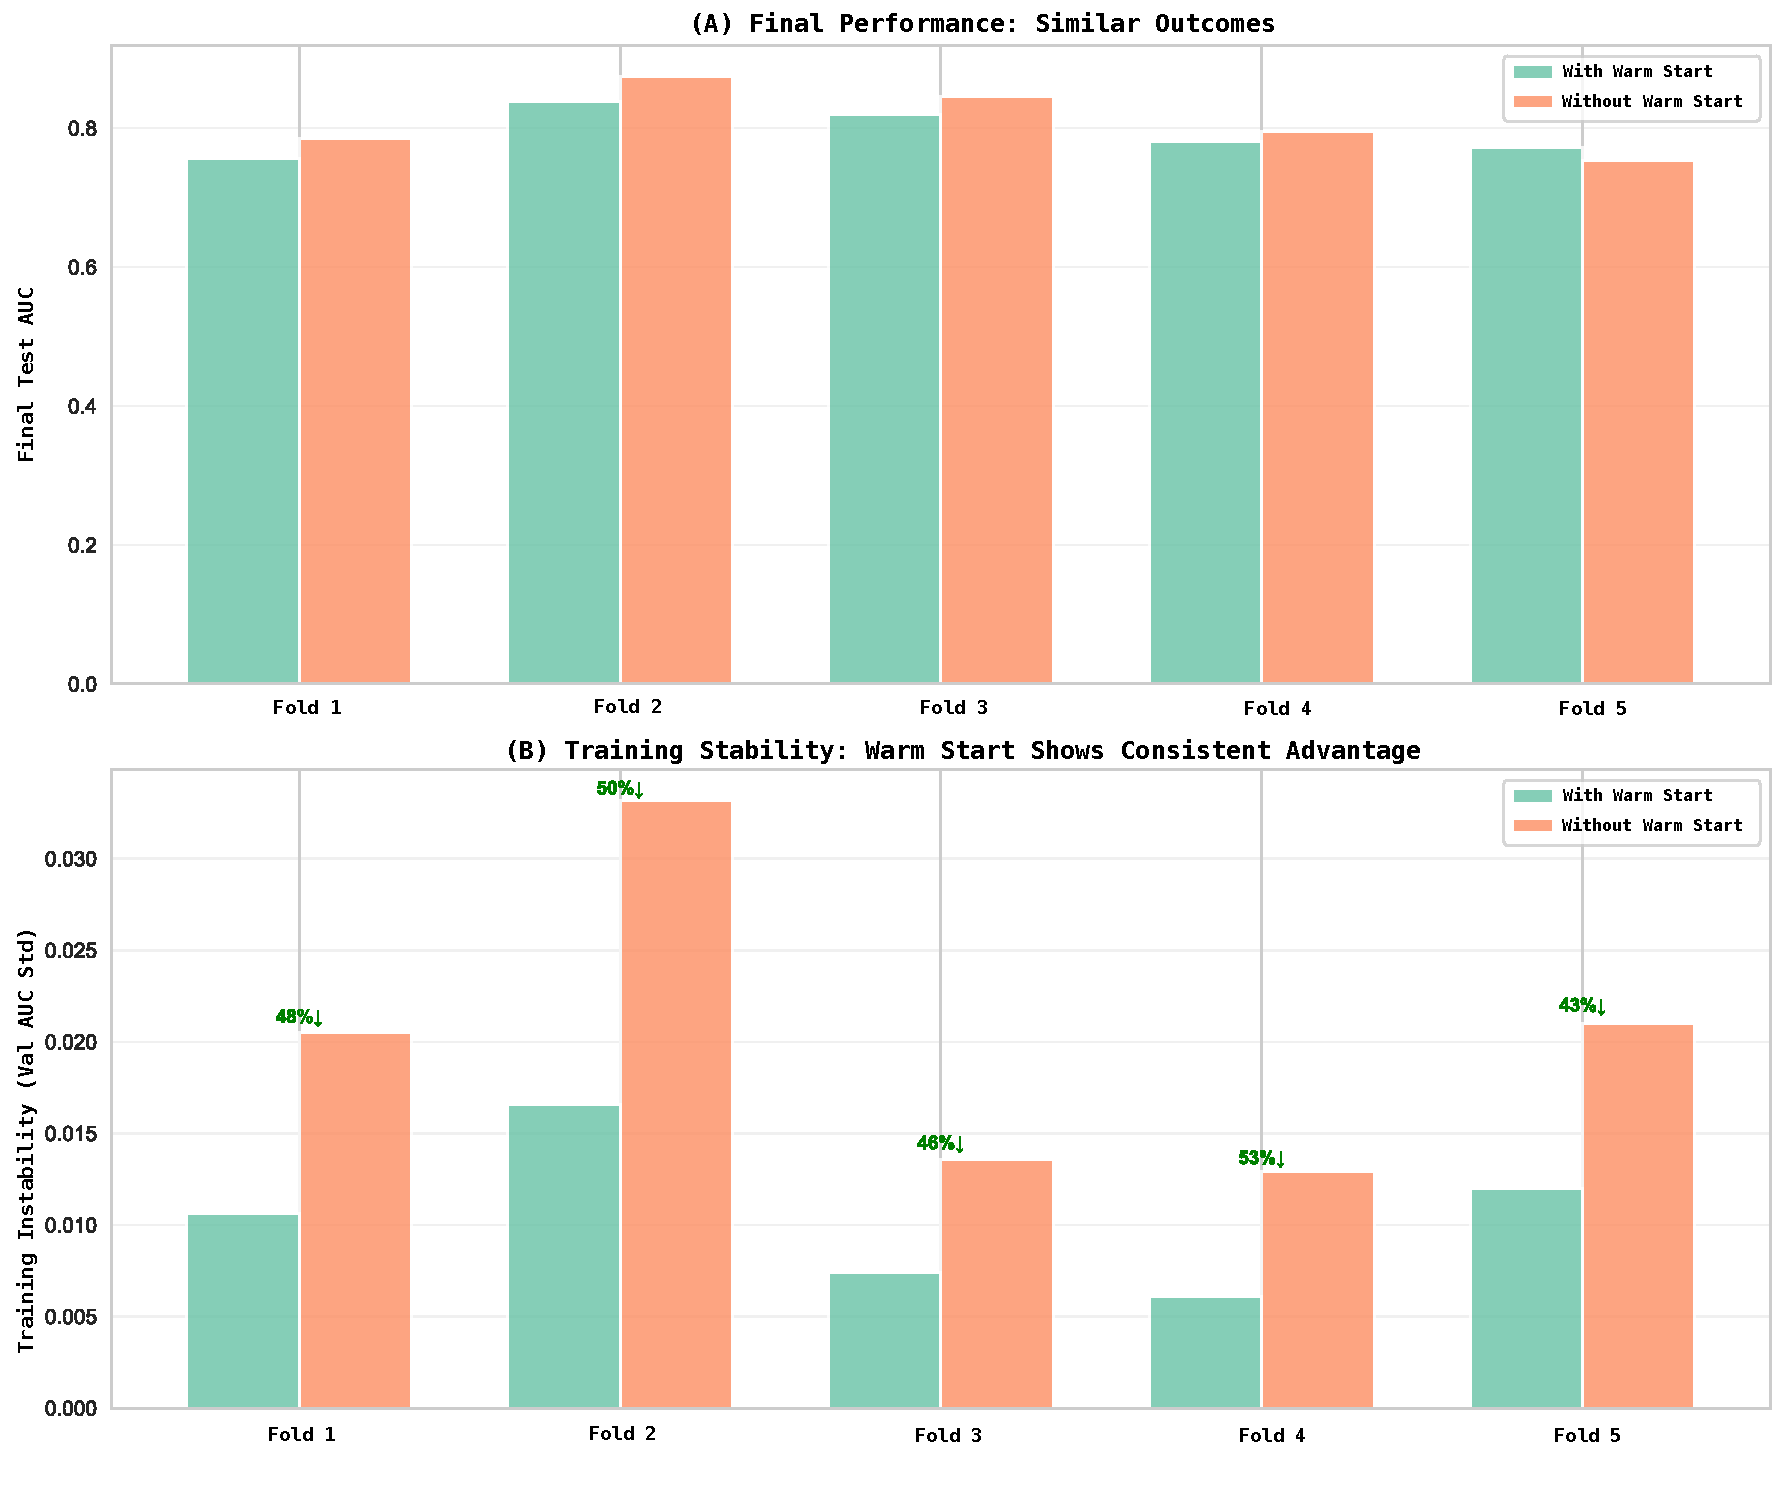
\includegraphics[width=0.8\linewidth]{figs/blca/warm_start/fold_wise_comparison.pdf}
    \caption{Impact of Warm Start on Training Stability and Final Performance. (A) Final test AUC across five folds remains comparable with and without warm start. (B) Warm start reduces training instablibity by 47.9\% on average, yielding more stable optimization trajectories and more predictable training outcomes.}
    \label{fig:warmstart_fold_wise_comparison}
\end{figure}

\clearpage
\section{Rationale for Slide-Level Routing}
\label{slide-level reasons}
CoR-Fuse performs routing at the slide level rather than the patch level because the objective of the router is to estimate the relative contribution of different foundation models for a given diagnostic task, rather than to identify discriminative tissue regions. First, the available supervision is provided only at the slide level, where each WSI is associated with a single diagnostic label. Patch-level routing would require learning \(P\times M\) encoder preferences for individual patches without direct patch-level supervision, potentially introducing additional uncertainty.

Second, our analysis in Section 3 focuses on slide-level encoder relationships and demonstrates that foundation-model contributions vary across slides rather than explicitly across tissue regions. Extending routing to the patch level would therefore require additional evidence for region-dependent encoder specialization.

Third, slide-level routing naturally complements MIL-based downstream architectures. Specifically, CoR-Fuse estimates which foundation models are informative for a slide, while the MIL attention module identifies which patches are relevant for prediction. Patch-level routing would couple encoder weighting with instance selection, potentially introducing unnecessary interaction between the two optimization processes.

Finally, slide-level routing substantially reduces the number of routing decisions. For a slide with \(P_n\) patches and \(M\) encoders, slide-level routing produces \(M\) encoder weights that are shared across patches, whereas patch-level routing requires \(P_n\times M\) routing scores. This design therefore provides a simpler and computationally more efficient routing mechanism while remaining compatible with the coordinate-aligned patch representations used for fusion. Patch-level adaptive routing, which could capture region-dependent encoder specialization, remains an interesting direction for future investigation.